\documentclass[tikz,border=5mm]{standalone}
\usetikzlibrary{arrows, decorations.pathmorphing, backgrounds, positioning, fit, petri}
\begin{document}

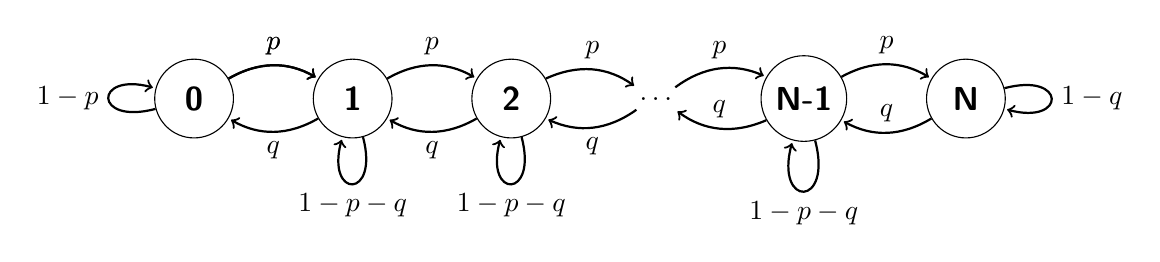
\begin{tikzpicture}
[state/.style={minimum size=1cm, circle,draw,font=\sffamily\large\bfseries}]

% NODES
\node [state] 	(0)  				{0};
\node [state] 	(1) [right=of 0]	{1};
\node [state] 	(2) [right=of 1]	{2};
\node [     ]   (3) [right=of 2]    {$\ldots$};
\node [state]   (4) [right=of 3]    {N-1};
\node [state]   (5) [right=of 4]    {N};
        
\path [thick,shorten >=1pt,auto]
(0) edge [->, loop left ] node [left]  {$1 - p$}     (0)
(0) edge [->, bend left ] node [above] {$p$}         (1)
(1) edge [->, loop below] node [below] {$1 - p - q$} (1)
(2) edge [->, loop below] node [below] {$1 - p - q$} (2)
(4) edge [->, loop below] node [below] {$1 - p - q$} (4)
(5) edge [->, loop right] node [right] {$1 - q$}     (5)
(0) edge [->, bend left ] node [above] {$p$}         (1)
(1) edge [->, bend left ] node [above] {$p$}         (2)
(2) edge [->, bend left ] node [above] {$p$}         (3)
(1) edge [->, bend left ] node [below] {$q$}         (0)
(2) edge [->, bend left ] node [below] {$q$}         (1)
(3) edge [->, bend left ] node [below] {$q$}         (2)
(3) edge [->, bend left ] node [above] {$p$}         (4)
(4) edge [->, bend left ] node [above] {$p$}         (5)
(5) edge [->, bend left ] node [above] {$q$}         (4)
(4) edge [->, bend left ] node [above] {$q$}         (3)
;

\end{tikzpicture}


\end{document}